\documentclass[twoside]{book}

% Packages required by doxygen
\usepackage{fixltx2e}
\usepackage{calc}
\usepackage{doxygen}
\usepackage[export]{adjustbox} % also loads graphicx
\usepackage{graphicx}
\usepackage[utf8]{inputenc}
\usepackage{makeidx}
\usepackage{multicol}
\usepackage{multirow}
\PassOptionsToPackage{warn}{textcomp}
\usepackage{textcomp}
\usepackage[nointegrals]{wasysym}
\usepackage[table]{xcolor}

% Font selection
\usepackage[T1]{fontenc}
\usepackage[scaled=.90]{helvet}
\usepackage{courier}
\usepackage{amssymb}
\usepackage{sectsty}
\renewcommand{\familydefault}{\sfdefault}
\allsectionsfont{%
  \fontseries{bc}\selectfont%
  \color{darkgray}%
}
\renewcommand{\DoxyLabelFont}{%
  \fontseries{bc}\selectfont%
  \color{darkgray}%
}
\newcommand{\+}{\discretionary{\mbox{\scriptsize$\hookleftarrow$}}{}{}}

% Page & text layout
\usepackage{geometry}
\geometry{%
  a4paper,%
  top=2.5cm,%
  bottom=2.5cm,%
  left=2.5cm,%
  right=2.5cm%
}
\tolerance=750
\hfuzz=15pt
\hbadness=750
\setlength{\emergencystretch}{15pt}
\setlength{\parindent}{0cm}
\setlength{\parskip}{3ex plus 2ex minus 2ex}
\makeatletter
\renewcommand{\paragraph}{%
  \@startsection{paragraph}{4}{0ex}{-1.0ex}{1.0ex}{%
    \normalfont\normalsize\bfseries\SS@parafont%
  }%
}
\renewcommand{\subparagraph}{%
  \@startsection{subparagraph}{5}{0ex}{-1.0ex}{1.0ex}{%
    \normalfont\normalsize\bfseries\SS@subparafont%
  }%
}
\makeatother

% Headers & footers
\usepackage{fancyhdr}
\pagestyle{fancyplain}
\fancyhead[LE]{\fancyplain{}{\bfseries\thepage}}
\fancyhead[CE]{\fancyplain{}{}}
\fancyhead[RE]{\fancyplain{}{\bfseries\leftmark}}
\fancyhead[LO]{\fancyplain{}{\bfseries\rightmark}}
\fancyhead[CO]{\fancyplain{}{}}
\fancyhead[RO]{\fancyplain{}{\bfseries\thepage}}
\fancyfoot[LE]{\fancyplain{}{}}
\fancyfoot[CE]{\fancyplain{}{}}
\fancyfoot[RE]{\fancyplain{}{\bfseries\scriptsize Generated by Doxygen }}
\fancyfoot[LO]{\fancyplain{}{\bfseries\scriptsize Generated by Doxygen }}
\fancyfoot[CO]{\fancyplain{}{}}
\fancyfoot[RO]{\fancyplain{}{}}
\renewcommand{\footrulewidth}{0.4pt}
\renewcommand{\chaptermark}[1]{%
  \markboth{#1}{}%
}
\renewcommand{\sectionmark}[1]{%
  \markright{\thesection\ #1}%
}

% Indices & bibliography
\usepackage{natbib}
\usepackage[titles]{tocloft}
\setcounter{tocdepth}{3}
\setcounter{secnumdepth}{5}
\makeindex

% Hyperlinks (required, but should be loaded last)
\usepackage{ifpdf}
\ifpdf
  \usepackage[pdftex,pagebackref=true]{hyperref}
\else
  \usepackage[ps2pdf,pagebackref=true]{hyperref}
\fi
\hypersetup{%
  colorlinks=true,%
  linkcolor=blue,%
  citecolor=blue,%
  unicode%
}

% Custom commands
\newcommand{\clearemptydoublepage}{%
  \newpage{\pagestyle{empty}\cleardoublepage}%
}

\usepackage{caption}
\captionsetup{labelsep=space,justification=centering,font={bf},singlelinecheck=off,skip=4pt,position=top}

%===== C O N T E N T S =====

\begin{document}

% Titlepage & ToC
\hypersetup{pageanchor=false,
             bookmarksnumbered=true,
             pdfencoding=unicode
            }
\pagenumbering{roman}
\begin{titlepage}
\vspace*{7cm}
\begin{center}%
{\Large Http server }\\
\vspace*{1cm}
{\large Generated by Doxygen 1.8.11}\\
\end{center}
\end{titlepage}
\clearemptydoublepage
\tableofcontents
\clearemptydoublepage
\pagenumbering{arabic}
\hypersetup{pageanchor=true}

%--- Begin generated contents ---
\chapter{Class Index}
\section{Class List}
Here are the classes, structs, unions and interfaces with brief descriptions\+:\begin{DoxyCompactList}
\item\contentsline{section}{\hyperlink{classPlaces}{Places} \\*Defines a favourite place }{\pageref{classPlaces}}{}
\end{DoxyCompactList}

\chapter{File Index}
\section{File List}
Here is a list of all documented files with brief descriptions\+:\begin{DoxyCompactList}
\item\contentsline{section}{\hyperlink{main_8cpp}{main.\+cpp} \\*Main file }{\pageref{main_8cpp}}{}
\item\contentsline{section}{include/\hyperlink{jsonconverter_8h}{jsonconverter.\+h} \\*Module to convert data to Json string }{\pageref{jsonconverter_8h}}{}
\item\contentsline{section}{include/\hyperlink{places_8h}{places.\+h} \\*Information about favourite place }{\pageref{places_8h}}{}
\item\contentsline{section}{include/\hyperlink{tcp__server_8h}{tcp\+\_\+server.\+h} \\*H\+T\+TP server }{\pageref{tcp__server_8h}}{}
\end{DoxyCompactList}

\chapter{Class Documentation}
\hypertarget{classPlaces}{}\section{Places Class Reference}
\label{classPlaces}\index{Places@{Places}}


defines a favourite place  




{\ttfamily \#include $<$places.\+h$>$}

\subsection*{Public Member Functions}
\begin{DoxyCompactItemize}
\item 
\hyperlink{classPlaces_a0a783d7b0464dd121c69bd93f82f9b87}{Places} ()\hypertarget{classPlaces_a0a783d7b0464dd121c69bd93f82f9b87}{}\label{classPlaces_a0a783d7b0464dd121c69bd93f82f9b87}

\begin{DoxyCompactList}\small\item\em default constructor for \hyperlink{classPlaces}{Places} \end{DoxyCompactList}\item 
\hyperlink{classPlaces_a94a948ece8bfd7bdd52cc16ae55c94a5}{$\sim$\+Places} ()\hypertarget{classPlaces_a94a948ece8bfd7bdd52cc16ae55c94a5}{}\label{classPlaces_a94a948ece8bfd7bdd52cc16ae55c94a5}

\begin{DoxyCompactList}\small\item\em default public destructor for Place \end{DoxyCompactList}\item 
\hyperlink{classPlaces_a3a5489045fba012f7428a5a76daf5a81}{Places} (int id, string name, string location)
\begin{DoxyCompactList}\small\item\em Constructor of the class. \end{DoxyCompactList}\item 
int \hyperlink{classPlaces_a8cd15caa1703fd336bad897b1e2d53bb}{get\+\_\+id} ()
\begin{DoxyCompactList}\small\item\em get object id \end{DoxyCompactList}\item 
string \hyperlink{classPlaces_a4ef51a60e65d562d128993645fc6a6c4}{get\+\_\+name} ()
\begin{DoxyCompactList}\small\item\em get object id \end{DoxyCompactList}\item 
string \hyperlink{classPlaces_a5d087707074477867cea4a0010895b66}{get\+\_\+location} ()
\begin{DoxyCompactList}\small\item\em get object location \end{DoxyCompactList}\end{DoxyCompactItemize}


\subsection{Detailed Description}
defines a favourite place 

\subsection{Constructor \& Destructor Documentation}
\index{Places@{Places}!Places@{Places}}
\index{Places@{Places}!Places@{Places}}
\subsubsection[{\texorpdfstring{Places(int id, string name, string location)}{Places(int id, string name, string location)}}]{\setlength{\rightskip}{0pt plus 5cm}Places\+::\+Places (
\begin{DoxyParamCaption}
\item[{int}]{id, }
\item[{string}]{name, }
\item[{string}]{location}
\end{DoxyParamCaption}
)}\hypertarget{classPlaces_a3a5489045fba012f7428a5a76daf5a81}{}\label{classPlaces_a3a5489045fba012f7428a5a76daf5a81}


Constructor of the class. 


\begin{DoxyParams}{Parameters}
{\em id} & -\/ object id \\
\hline
{\em name} & -\/ object name \\
\hline
{\em location} & -\/ object location \\
\hline
\end{DoxyParams}


\subsection{Member Function Documentation}
\index{Places@{Places}!get\+\_\+id@{get\+\_\+id}}
\index{get\+\_\+id@{get\+\_\+id}!Places@{Places}}
\subsubsection[{\texorpdfstring{get\+\_\+id()}{get_id()}}]{\setlength{\rightskip}{0pt plus 5cm}int Places\+::get\+\_\+id (
\begin{DoxyParamCaption}
{}
\end{DoxyParamCaption}
)}\hypertarget{classPlaces_a8cd15caa1703fd336bad897b1e2d53bb}{}\label{classPlaces_a8cd15caa1703fd336bad897b1e2d53bb}


get object id 

\begin{DoxyReturn}{Returns}
unique number of Place 
\end{DoxyReturn}
\index{Places@{Places}!get\+\_\+location@{get\+\_\+location}}
\index{get\+\_\+location@{get\+\_\+location}!Places@{Places}}
\subsubsection[{\texorpdfstring{get\+\_\+location()}{get_location()}}]{\setlength{\rightskip}{0pt plus 5cm}string Places\+::get\+\_\+location (
\begin{DoxyParamCaption}
{}
\end{DoxyParamCaption}
)}\hypertarget{classPlaces_a5d087707074477867cea4a0010895b66}{}\label{classPlaces_a5d087707074477867cea4a0010895b66}


get object location 

\begin{DoxyReturn}{Returns}
location of Place 
\end{DoxyReturn}
\index{Places@{Places}!get\+\_\+name@{get\+\_\+name}}
\index{get\+\_\+name@{get\+\_\+name}!Places@{Places}}
\subsubsection[{\texorpdfstring{get\+\_\+name()}{get_name()}}]{\setlength{\rightskip}{0pt plus 5cm}string Places\+::get\+\_\+name (
\begin{DoxyParamCaption}
{}
\end{DoxyParamCaption}
)}\hypertarget{classPlaces_a4ef51a60e65d562d128993645fc6a6c4}{}\label{classPlaces_a4ef51a60e65d562d128993645fc6a6c4}


get object id 

\begin{DoxyReturn}{Returns}
name of Place 
\end{DoxyReturn}


The documentation for this class was generated from the following files\+:\begin{DoxyCompactItemize}
\item 
include/\hyperlink{places_8h}{places.\+h}\item 
src/places.\+cpp\end{DoxyCompactItemize}

\chapter{File Documentation}
\hypertarget{jsonconverter_8h}{}\section{include/jsonconverter.h File Reference}
\label{jsonconverter_8h}\index{include/jsonconverter.\+h@{include/jsonconverter.\+h}}


Module to convert data to Json string.  


{\ttfamily \#include $<$iostream$>$}\\*
{\ttfamily \#include $<$vector$>$}\\*
{\ttfamily \#include \char`\"{}places.\+h\char`\"{}}\\*
Include dependency graph for jsonconverter.\+h\+:
\nopagebreak
\begin{figure}[H]
\begin{center}
\leavevmode
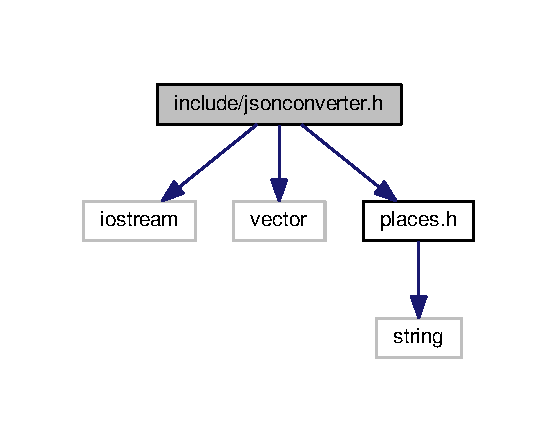
\includegraphics[width=268pt]{jsonconverter_8h__incl}
\end{center}
\end{figure}
\subsection*{Functions}
\begin{DoxyCompactItemize}
\item 
string \hyperlink{jsonconverter_8h_a9b4369d668f311c1f5fcdc600956281a}{server\+Information} (string servername, string developer)
\begin{DoxyCompactList}\small\item\em get server information \end{DoxyCompactList}\item 
string \hyperlink{jsonconverter_8h_a6ed6ea0595329e4606cb4d7fcf4cb6db}{my\+Favourite\+Places} (vector$<$ \hyperlink{classPlaces}{Places} $\ast$ $>$ place)
\begin{DoxyCompactList}\small\item\em get all places in Json fromat \end{DoxyCompactList}\item 
string \hyperlink{jsonconverter_8h_ad38a7250e0295df6f6057b4dde1a49f4}{location\+Place} (vector$<$ \hyperlink{classPlaces}{Places} $\ast$ $>$ place, string message)
\begin{DoxyCompactList}\small\item\em get information about my favourites places with some location \end{DoxyCompactList}\item 
string \hyperlink{jsonconverter_8h_a3f8e63cd7d4edd3c7108eae9acf74aec}{id\+Place} (vector$<$ \hyperlink{classPlaces}{Places} $\ast$ $>$ place, string message)
\begin{DoxyCompactList}\small\item\em get information about my favourites places with some id \end{DoxyCompactList}\item 
string \hyperlink{jsonconverter_8h_a6bb4a7d88b588add9c542426d5a2fe10}{file\+Information} ()
\begin{DoxyCompactList}\small\item\em Take data from file. \end{DoxyCompactList}\item 
string \hyperlink{jsonconverter_8h_a7160388c00905eb853fc867ca9d31ca5}{file\+Letters} ()
\begin{DoxyCompactList}\small\item\em Calculate letters in Upper register and in Lower. \end{DoxyCompactList}\end{DoxyCompactItemize}


\subsection{Detailed Description}
Module to convert data to Json string. 



\subsection{Function Documentation}
\index{jsonconverter.\+h@{jsonconverter.\+h}!file\+Information@{file\+Information}}
\index{file\+Information@{file\+Information}!jsonconverter.\+h@{jsonconverter.\+h}}
\subsubsection[{\texorpdfstring{file\+Information()}{fileInformation()}}]{\setlength{\rightskip}{0pt plus 5cm}string file\+Information (
\begin{DoxyParamCaption}
{}
\end{DoxyParamCaption}
)}\hypertarget{jsonconverter_8h_a6bb4a7d88b588add9c542426d5a2fe10}{}\label{jsonconverter_8h_a6bb4a7d88b588add9c542426d5a2fe10}


Take data from file. 

\begin{DoxyReturn}{Returns}
json string which contains information about file size, file name and file data 
\end{DoxyReturn}
\index{jsonconverter.\+h@{jsonconverter.\+h}!file\+Letters@{file\+Letters}}
\index{file\+Letters@{file\+Letters}!jsonconverter.\+h@{jsonconverter.\+h}}
\subsubsection[{\texorpdfstring{file\+Letters()}{fileLetters()}}]{\setlength{\rightskip}{0pt plus 5cm}string file\+Letters (
\begin{DoxyParamCaption}
{}
\end{DoxyParamCaption}
)}\hypertarget{jsonconverter_8h_a7160388c00905eb853fc867ca9d31ca5}{}\label{jsonconverter_8h_a7160388c00905eb853fc867ca9d31ca5}


Calculate letters in Upper register and in Lower. 

\begin{DoxyReturn}{Returns}
information about letters in Upper register and in Lower 
\end{DoxyReturn}
\index{jsonconverter.\+h@{jsonconverter.\+h}!id\+Place@{id\+Place}}
\index{id\+Place@{id\+Place}!jsonconverter.\+h@{jsonconverter.\+h}}
\subsubsection[{\texorpdfstring{id\+Place(vector$<$ Places $\ast$ $>$ place, string message)}{idPlace(vector< Places * > place, string message)}}]{\setlength{\rightskip}{0pt plus 5cm}string id\+Place (
\begin{DoxyParamCaption}
\item[{vector$<$ {\bf Places} $\ast$ $>$}]{place, }
\item[{string}]{message}
\end{DoxyParamCaption}
)}\hypertarget{jsonconverter_8h_a3f8e63cd7d4edd3c7108eae9acf74aec}{}\label{jsonconverter_8h_a3f8e63cd7d4edd3c7108eae9acf74aec}


get information about my favourites places with some id 


\begin{DoxyParams}{Parameters}
{\em place} & -\/ the vector with my favourite places \\
\hline
{\em message} & -\/ H\+T\+TP request to server \\
\hline
\end{DoxyParams}
\begin{DoxyReturn}{Returns}
json string which contains information about place with selected id 
\end{DoxyReturn}
\index{jsonconverter.\+h@{jsonconverter.\+h}!location\+Place@{location\+Place}}
\index{location\+Place@{location\+Place}!jsonconverter.\+h@{jsonconverter.\+h}}
\subsubsection[{\texorpdfstring{location\+Place(vector$<$ Places $\ast$ $>$ place, string message)}{locationPlace(vector< Places * > place, string message)}}]{\setlength{\rightskip}{0pt plus 5cm}string location\+Place (
\begin{DoxyParamCaption}
\item[{vector$<$ {\bf Places} $\ast$ $>$}]{place, }
\item[{string}]{message}
\end{DoxyParamCaption}
)}\hypertarget{jsonconverter_8h_ad38a7250e0295df6f6057b4dde1a49f4}{}\label{jsonconverter_8h_ad38a7250e0295df6f6057b4dde1a49f4}


get information about my favourites places with some location 


\begin{DoxyParams}{Parameters}
{\em place} & -\/ the vector with my favourite places \\
\hline
{\em message} & -\/ H\+T\+TP request to server \\
\hline
\end{DoxyParams}
\begin{DoxyReturn}{Returns}
json string which contains information about selected places 
\end{DoxyReturn}
\index{jsonconverter.\+h@{jsonconverter.\+h}!my\+Favourite\+Places@{my\+Favourite\+Places}}
\index{my\+Favourite\+Places@{my\+Favourite\+Places}!jsonconverter.\+h@{jsonconverter.\+h}}
\subsubsection[{\texorpdfstring{my\+Favourite\+Places(vector$<$ Places $\ast$ $>$ place)}{myFavouritePlaces(vector< Places * > place)}}]{\setlength{\rightskip}{0pt plus 5cm}string my\+Favourite\+Places (
\begin{DoxyParamCaption}
\item[{vector$<$ {\bf Places} $\ast$ $>$}]{place}
\end{DoxyParamCaption}
)}\hypertarget{jsonconverter_8h_a6ed6ea0595329e4606cb4d7fcf4cb6db}{}\label{jsonconverter_8h_a6ed6ea0595329e4606cb4d7fcf4cb6db}


get all places in Json fromat 


\begin{DoxyParams}{Parameters}
{\em place} & -\/ vector of my favourites \hyperlink{classPlaces}{Places} \\
\hline
\end{DoxyParams}
\begin{DoxyReturn}{Returns}
string in Json format that contain information about all places 
\end{DoxyReturn}
\index{jsonconverter.\+h@{jsonconverter.\+h}!server\+Information@{server\+Information}}
\index{server\+Information@{server\+Information}!jsonconverter.\+h@{jsonconverter.\+h}}
\subsubsection[{\texorpdfstring{server\+Information(string servername, string developer)}{serverInformation(string servername, string developer)}}]{\setlength{\rightskip}{0pt plus 5cm}string server\+Information (
\begin{DoxyParamCaption}
\item[{string}]{servername, }
\item[{string}]{developer}
\end{DoxyParamCaption}
)}\hypertarget{jsonconverter_8h_a9b4369d668f311c1f5fcdc600956281a}{}\label{jsonconverter_8h_a9b4369d668f311c1f5fcdc600956281a}


get server information 

\begin{DoxyReturn}{Returns}
Json string that contains information about server 
\end{DoxyReturn}

\hypertarget{places_8h}{}\section{include/places.h File Reference}
\label{places_8h}\index{include/places.\+h@{include/places.\+h}}


Information about favourite place.  


{\ttfamily \#include $<$string$>$}\\*
Include dependency graph for places.\+h\+:
\nopagebreak
\begin{figure}[H]
\begin{center}
\leavevmode
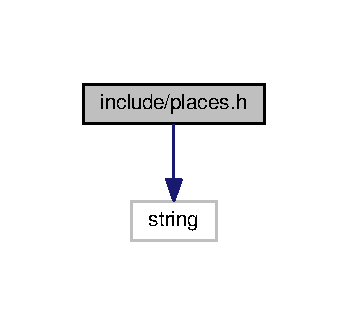
\includegraphics[width=167pt]{places_8h__incl}
\end{center}
\end{figure}
This graph shows which files directly or indirectly include this file\+:
\nopagebreak
\begin{figure}[H]
\begin{center}
\leavevmode
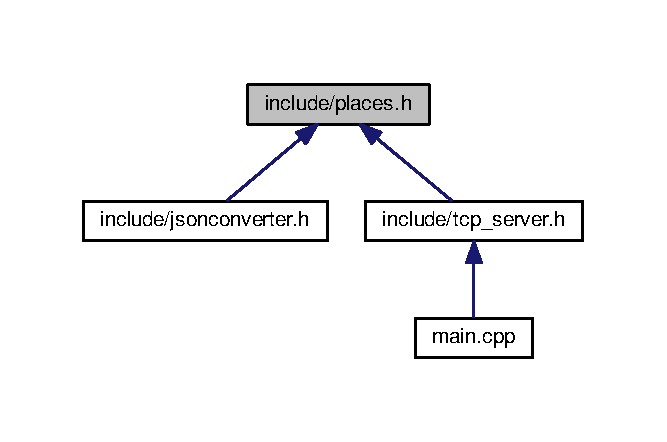
\includegraphics[width=320pt]{places_8h__dep__incl}
\end{center}
\end{figure}
\subsection*{Classes}
\begin{DoxyCompactItemize}
\item 
class \hyperlink{classPlaces}{Places}
\begin{DoxyCompactList}\small\item\em defines a favourite place \end{DoxyCompactList}\end{DoxyCompactItemize}


\subsection{Detailed Description}
Information about favourite place. 


\hypertarget{tcp__server_8h}{}\section{include/tcp\+\_\+server.h File Reference}
\label{tcp__server_8h}\index{include/tcp\+\_\+server.\+h@{include/tcp\+\_\+server.\+h}}


H\+T\+TP server.  


{\ttfamily \#include $<$progbase-\/cpp/net.\+h$>$}\\*
{\ttfamily \#include $<$iostream$>$}\\*
{\ttfamily \#include $<$vector$>$}\\*
{\ttfamily \#include \char`\"{}places.\+h\char`\"{}}\\*
{\ttfamily \#include $<$ctype.\+h$>$}\\*
{\ttfamily \#include $<$string$>$}\\*
Include dependency graph for tcp\+\_\+server.\+h\+:
\nopagebreak
\begin{figure}[H]
\begin{center}
\leavevmode
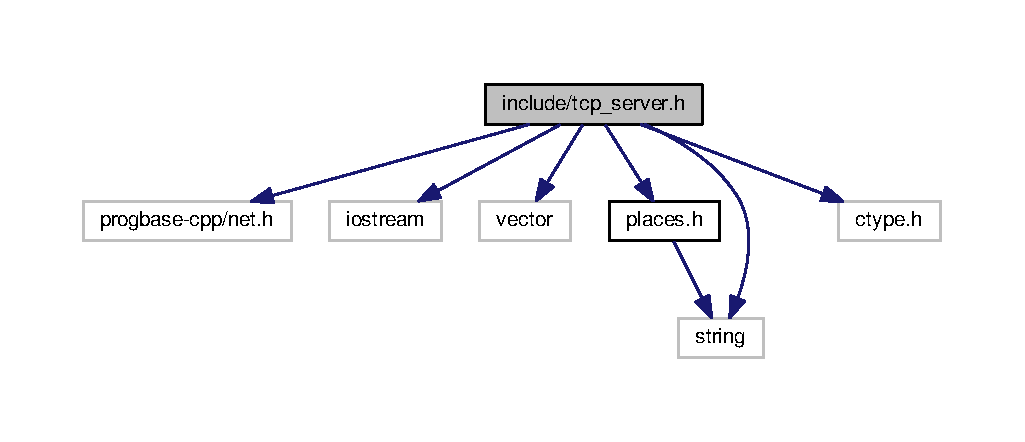
\includegraphics[width=350pt]{tcp__server_8h__incl}
\end{center}
\end{figure}
This graph shows which files directly or indirectly include this file\+:
\nopagebreak
\begin{figure}[H]
\begin{center}
\leavevmode
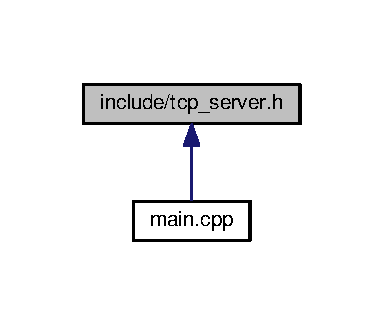
\includegraphics[width=184pt]{tcp__server_8h__dep__incl}
\end{center}
\end{figure}
\subsection*{Functions}
\begin{DoxyCompactItemize}
\item 
int \hyperlink{tcp__server_8h_acb23214d995eb273b364ca7bac1abff2}{tcp\+Server} ()
\begin{DoxyCompactList}\small\item\em H\+T\+TP server. \end{DoxyCompactList}\end{DoxyCompactItemize}


\subsection{Detailed Description}
H\+T\+TP server. 



\subsection{Function Documentation}
\index{tcp\+\_\+server.\+h@{tcp\+\_\+server.\+h}!tcp\+Server@{tcp\+Server}}
\index{tcp\+Server@{tcp\+Server}!tcp\+\_\+server.\+h@{tcp\+\_\+server.\+h}}
\subsubsection[{\texorpdfstring{tcp\+Server()}{tcpServer()}}]{\setlength{\rightskip}{0pt plus 5cm}int tcp\+Server (
\begin{DoxyParamCaption}
{}
\end{DoxyParamCaption}
)}\hypertarget{tcp__server_8h_acb23214d995eb273b364ca7bac1abff2}{}\label{tcp__server_8h_acb23214d995eb273b364ca7bac1abff2}


H\+T\+TP server. 

\begin{DoxyReturn}{Returns}
exit success 
\end{DoxyReturn}

\hypertarget{main_8cpp}{}\section{main.\+cpp File Reference}
\label{main_8cpp}\index{main.\+cpp@{main.\+cpp}}


main file  


{\ttfamily \#include $<$iostream$>$}\\*
{\ttfamily \#include \char`\"{}tcp\+\_\+server.\+h\char`\"{}}\\*
{\ttfamily \#include $<$fstream$>$}\\*
Include dependency graph for main.\+cpp\+:
\nopagebreak
\begin{figure}[H]
\begin{center}
\leavevmode
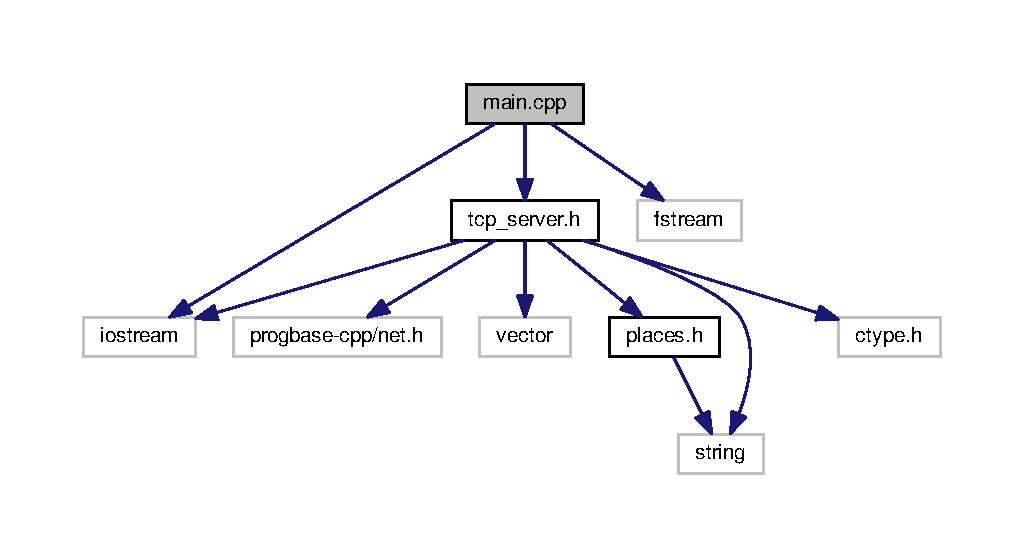
\includegraphics[width=350pt]{main_8cpp__incl}
\end{center}
\end{figure}
\subsection*{Functions}
\begin{DoxyCompactItemize}
\item 
int {\bfseries main} (void)\hypertarget{main_8cpp_a840291bc02cba5474a4cb46a9b9566fe}{}\label{main_8cpp_a840291bc02cba5474a4cb46a9b9566fe}

\end{DoxyCompactItemize}


\subsection{Detailed Description}
main file 


%--- End generated contents ---

% Index
\backmatter
\newpage
\phantomsection
\clearemptydoublepage
\addcontentsline{toc}{chapter}{Index}
\printindex

\end{document}
